\subsection{Correlation and Importance}

This subsection reports two descriptive analyses using different datasets.
First, we calculate Pearson correlations among the 77 observations in the \texttt{PWDriverFeatureSet} dataset, without isolation-forest filtering.
Second, we assess random-forest feature importance for plastic-waste generation using the \texttt{PWGPredictors} dataset.
An isolation forest fitted to the predictor variables, with a contamination setting of \(0.05\), flagged 31 of the 602 observations as potentially unusual; we excluded these observations and fitted the random forest to the remaining 571.
Neither analysis uses a train--test split.
The flagged observations are not necessarily errors, and we did not compare feature importance with and without filtering.
The importance results therefore describe this filtered fit and may depend on the filtering choice.

\begin{figure}[H]
	\centering
	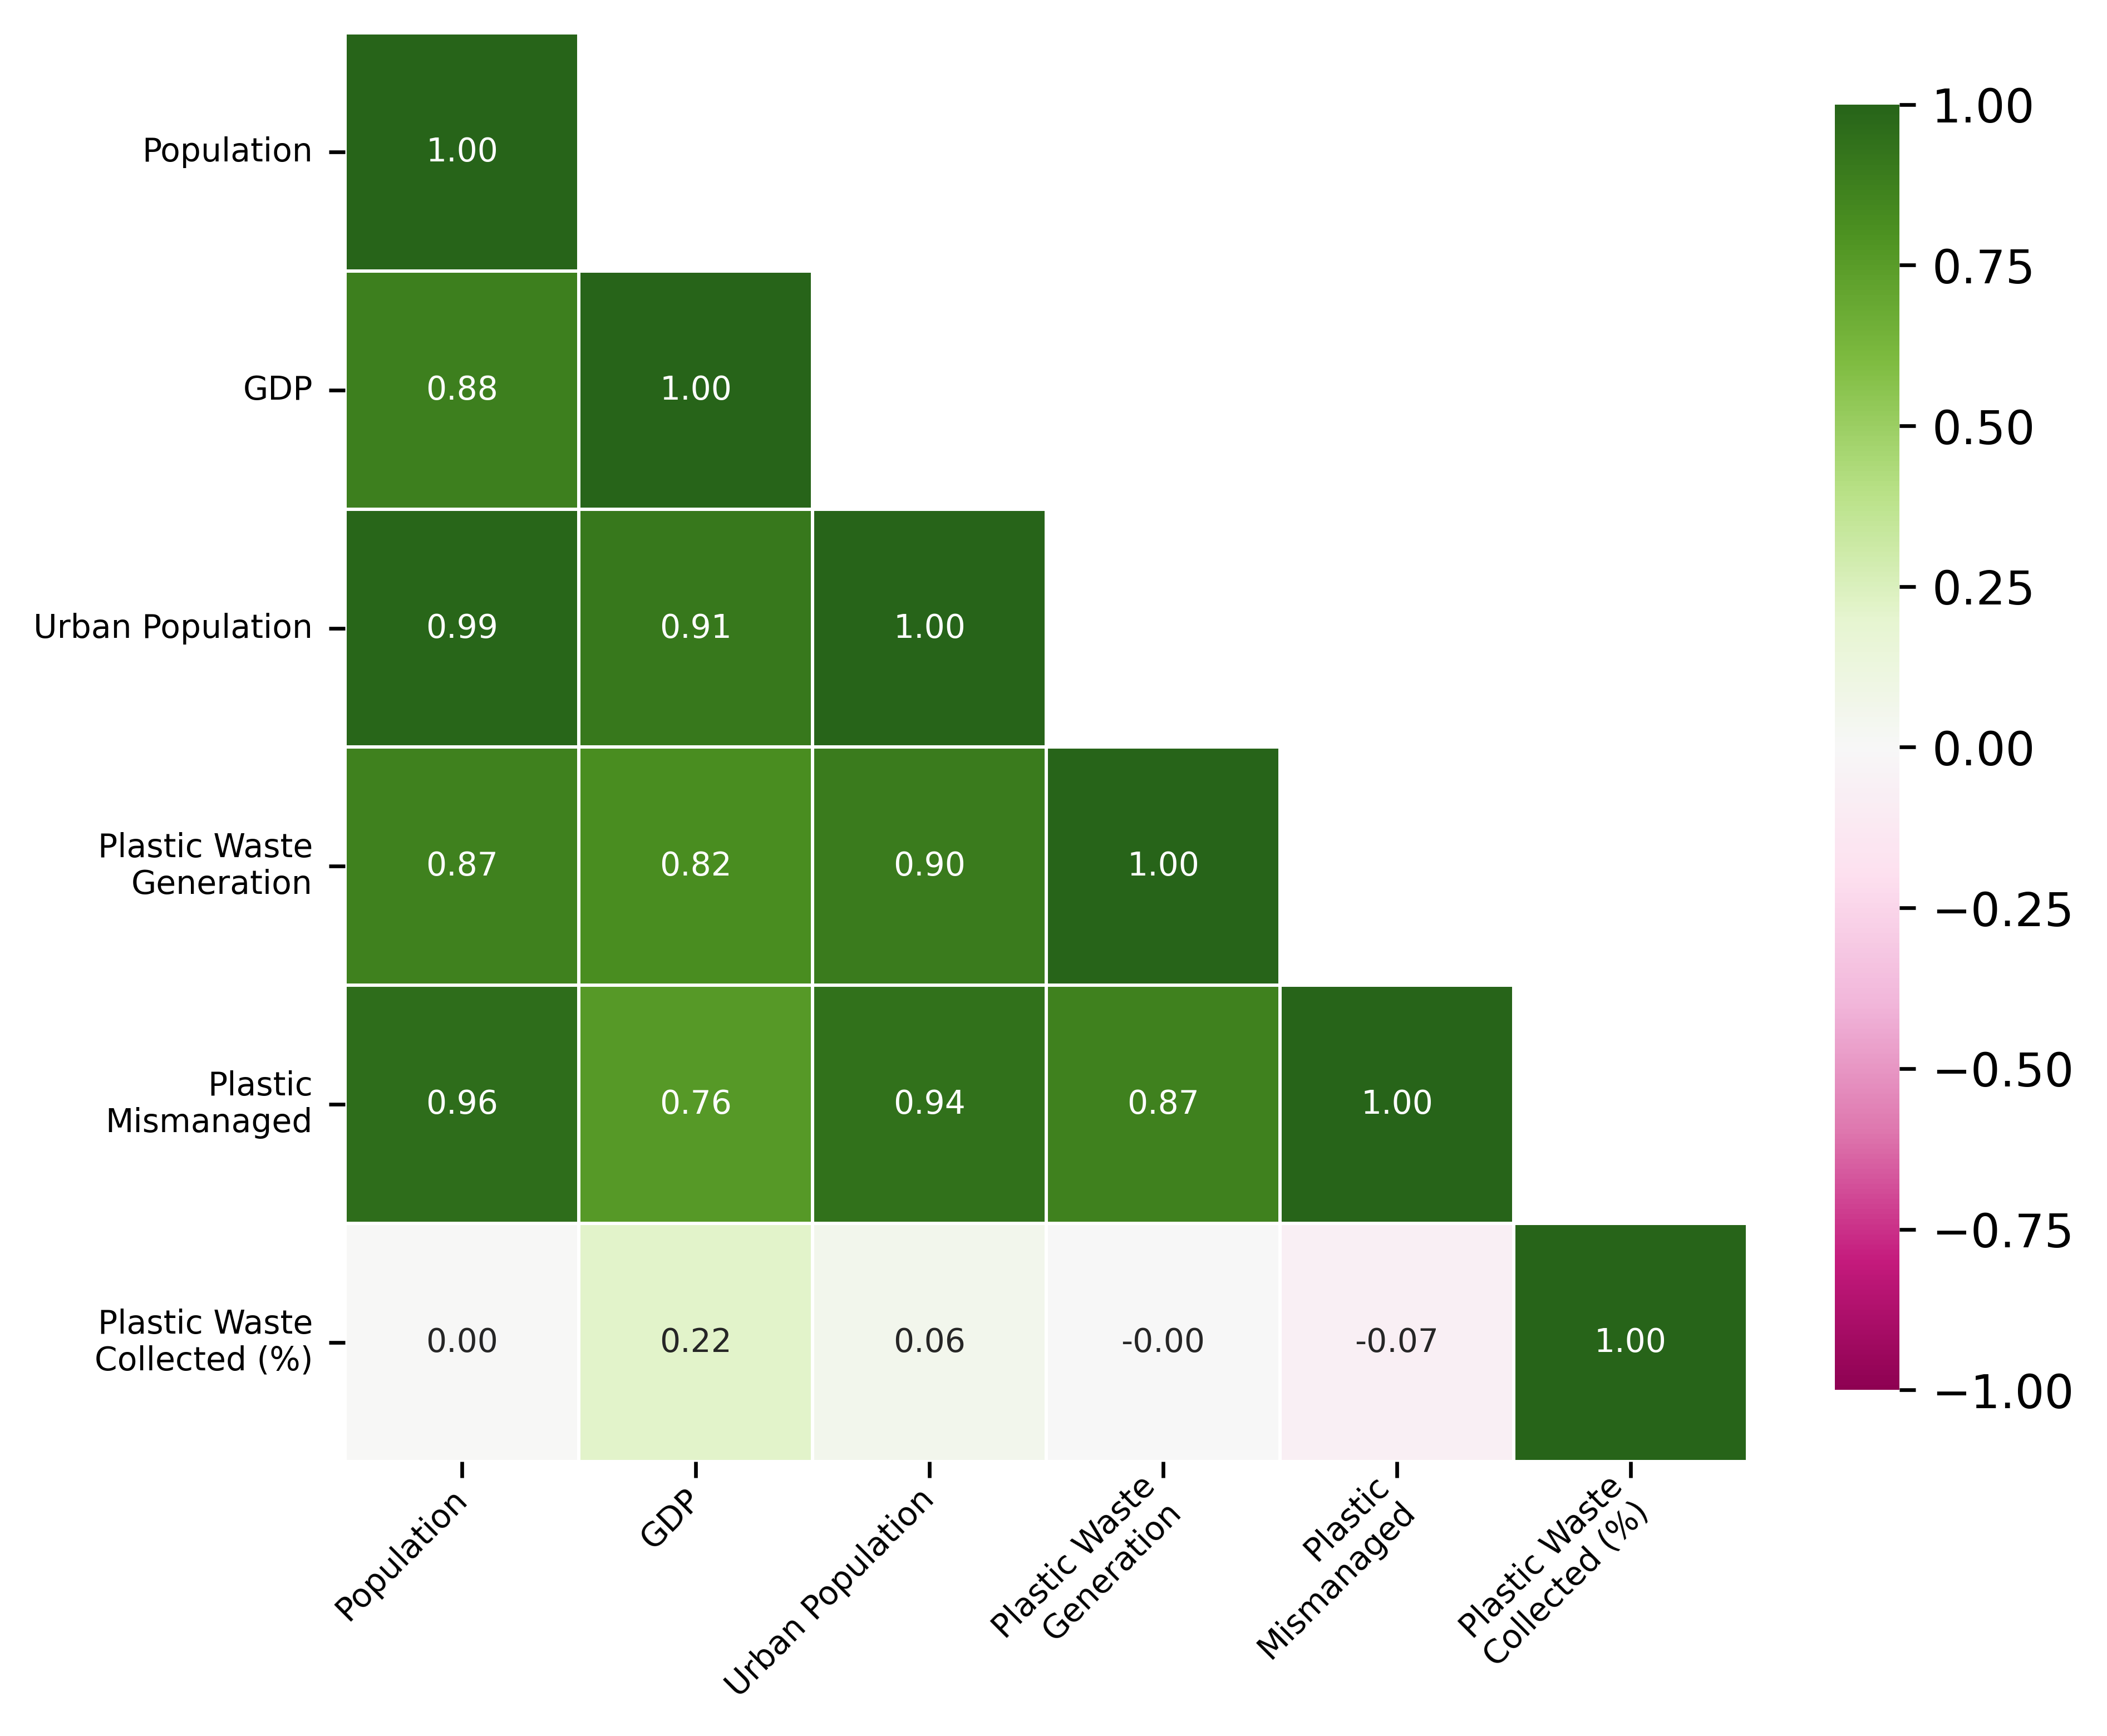
\includegraphics[width=0.9\linewidth]{figures/correlation_matrix.png}
	\caption{
		\centering
		Correlation matrix for the pooled \texttt{PWDriverFeatureSet} dataset. It summarizes pairwise association patterns across the pooled driver set.
	}
	\label{fig:correlation_matrix}
\end{figure}


Figure~\ref{fig:correlation_matrix} presents the resulting Pearson correlations.
Plastic waste generation was positively correlated with GDP \((r = 0.82)\).
Its correlation with urban population \((r = 0.90)\) was stronger than its correlation with total population \((r = 0.87)\).
Total population and mismanaged plastic waste were also strongly correlated \((r = 0.96)\).
In contrast, the percentage of plastic waste that was properly managed was nearly uncorrelated with variables measuring scale.
These associations may partly reflect differences in country size, since most variables represent national totals.
The pooled correlations do not distinguish cross-country differences from within-country changes or account for differences in measurement methods across the source data.
They should therefore be interpreted descriptively rather than causally.

\begin{figure}[H]
	\centering
	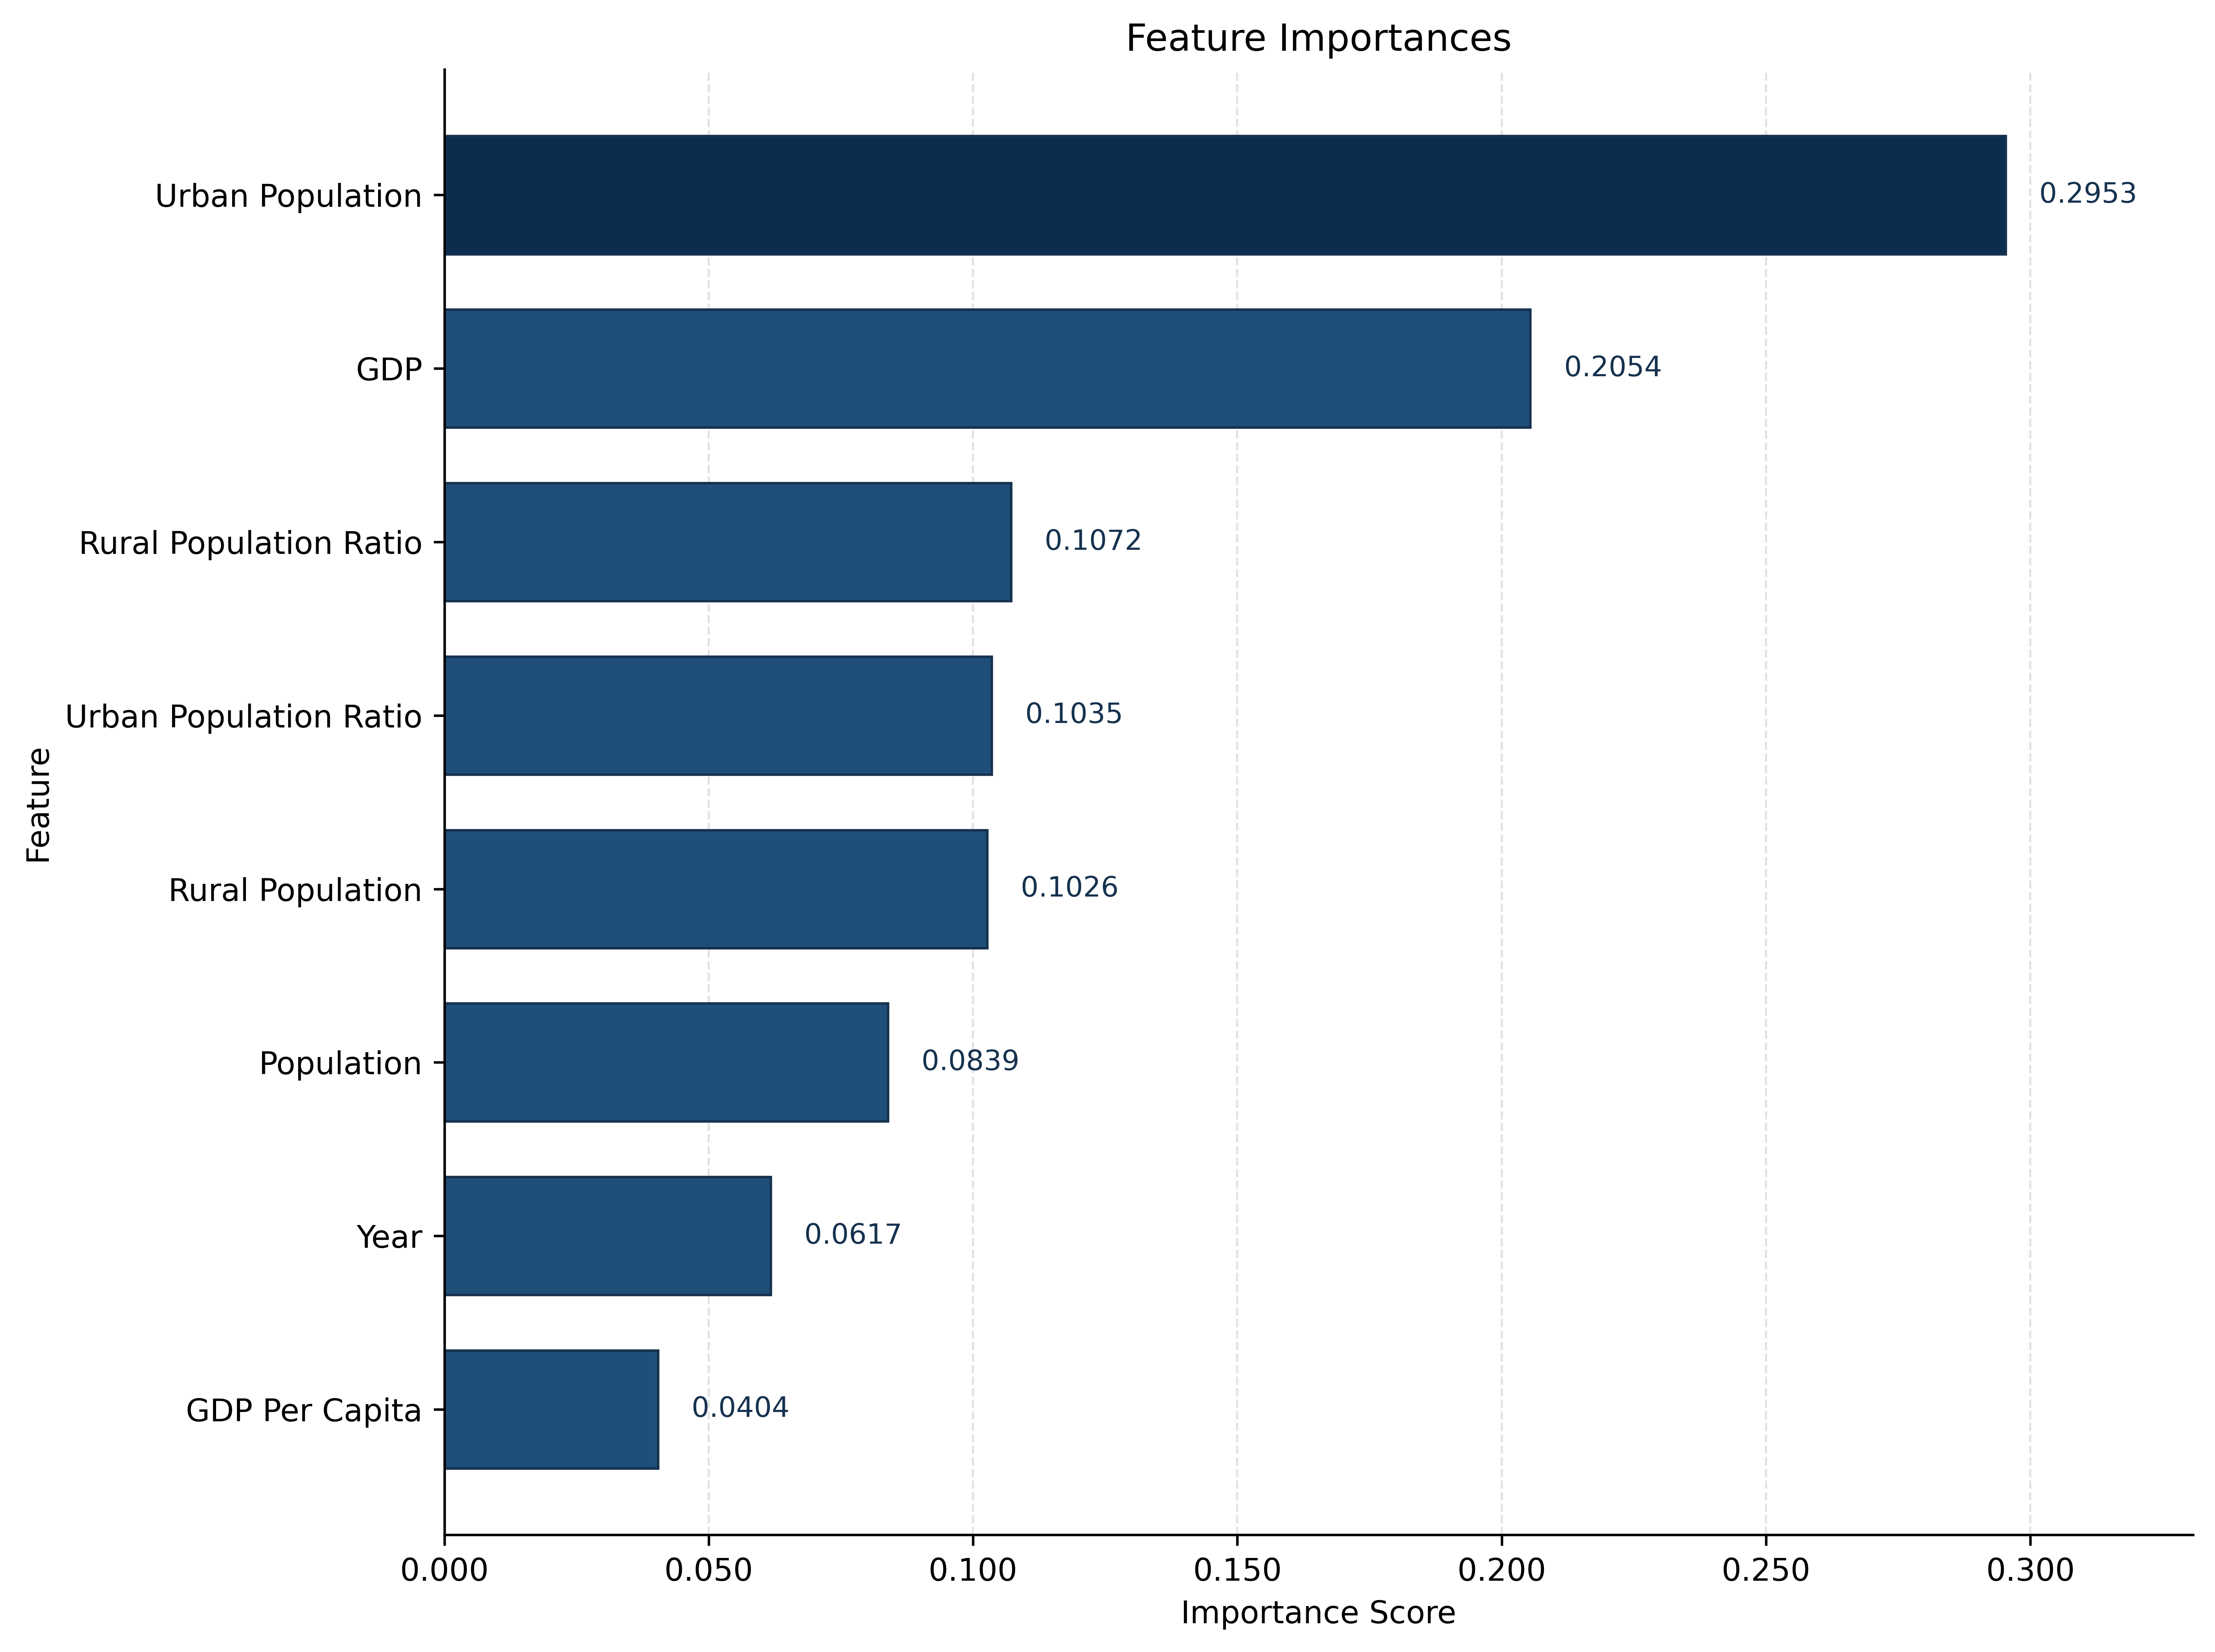
\includegraphics[width=1.0\linewidth]{figures/feature_importances.png}
	\caption{
		\centering
		Feature importances for the \texttt{PWGPredictors} dataset. This bar chart shows the relative importance of each feature in predicting plastic waste generation.
	}
	\label{fig:feature_importances}
\end{figure}


Figure~\ref{fig:feature_importances} presents the random-forest feature importances for predicting plastic-waste generation.
Urban population has the highest importance score \((0.2953)\), followed by GDP \((0.2054)\), rural population ratio \((0.1072)\), urban population ratio \((0.1035)\), rural population \((0.1026)\), population \((0.0839)\), year \((0.0617)\), and GDP per capita \((0.0404)\).
The correlation and impurity-based feature-importance analyses are descriptive and predictive rather than causal; their values may reflect country scale, temporal trends, correlated predictors, and source composition.
